\section{Genes in Regions of Anomalous GC Content}
\label{section:gc-regions}

Figure~\ref{fig:gc-regions} and Table \ref{table:gc-regions} shows the results of applying the same
region finding process from earlier to segments of the genome
identified as AT-rich. AT-rich is defined as a region of genomic
sequence with percent GC composition less than 28\% as determined in
Section \ref{section:assemblies}. In comparison to results from
Section \ref{section:regions}, we see that overall there are far fewer
regions with gene predictions in AT-rich genomic segments. In DC1,
Tsth20, there are very few regions with full support from both Braker2
and GeneMark, but more singletons. Again, as in Section
\ref{section:regions}, there are no regions with partial support as
only two gene finding tools were applied to those
assemblies. \textit{T. reesei} and \textit{T. harzianum} report more
regions in AT-rich genomic sequence than the other assemblies, but
with the majority of regions belonging to the singleton
category. \textit{T. virens} is an interesting case, reporting a
similar numbers of regions and genes in AT-rich genomic sequence as
DC1 and Tsth20. \textit{T. virens} is also the only assembly to report
zero singleton gene predictions. Why \textit{T. virens} differs from
the other RefSeq assemblies is unclear. In general, there are few
regions with gene predictions in AT-rich genomic segments, and within
these regions, the majority of cases are isolated singleton gene
predictions. These observations differ greatly from those made in
nucleotide composition agnostic approach in Section
\ref{section:regions}.

\begin{figure}
  \centering
  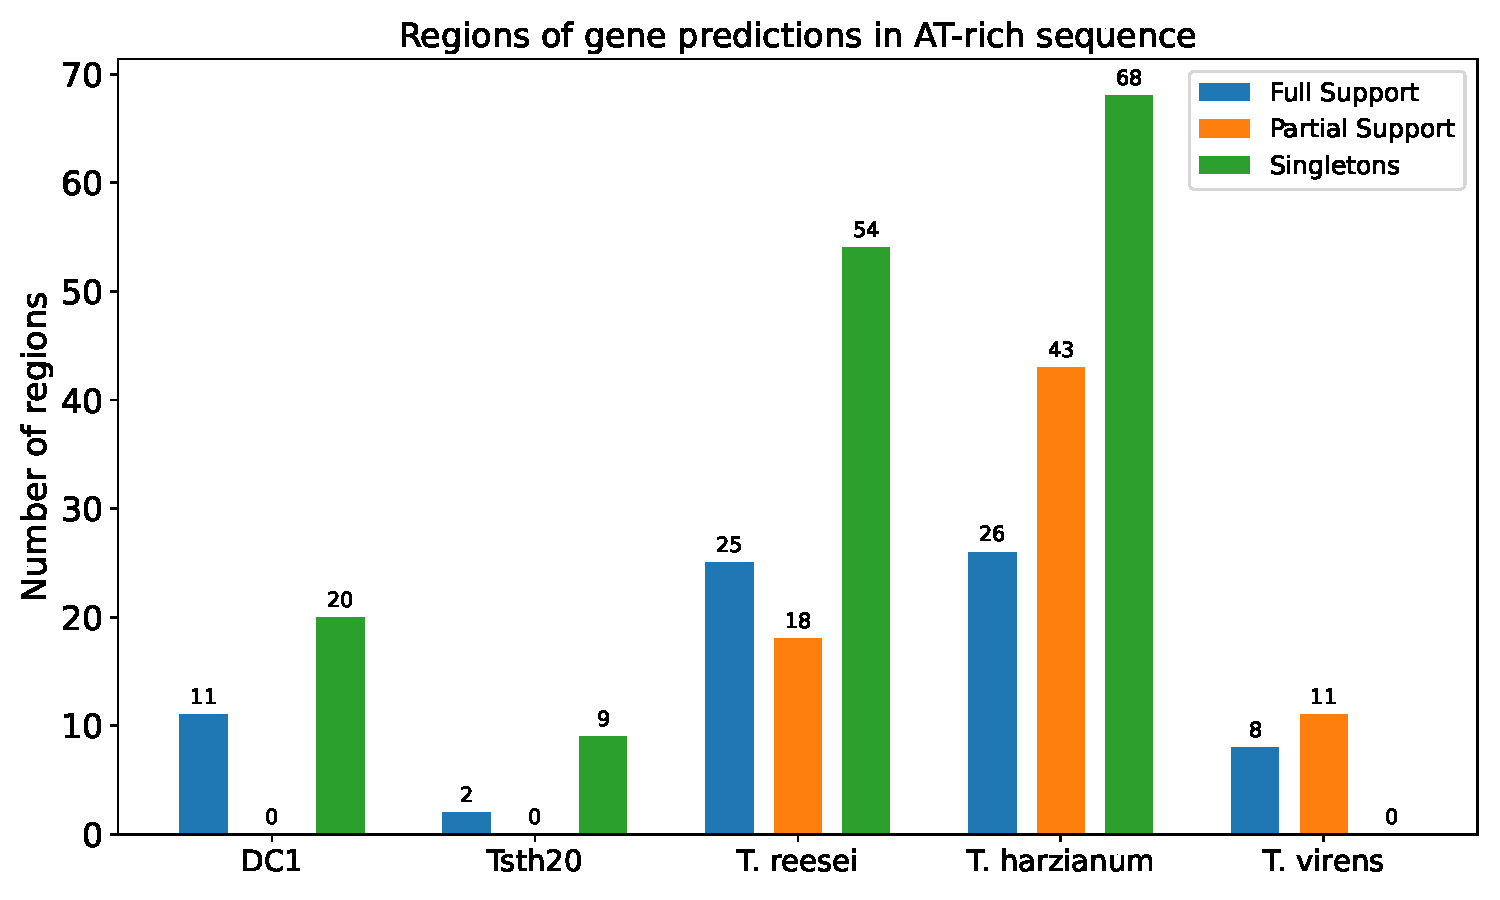
\includegraphics[width=0.90\textwidth]{figures/atrich-regions-barplot.pdf}
  \caption[Regions of agreement in AT-rich genomic sequence]{Regions of full, partial, and no agreement in AT-rich genomic sequence. It is important to note that in the cases of DC1 and Tsth20, full support indicates supporting gene predictions from both GeneMark and Braker2 and as such, there are no regions with partial support.}
  \label{fig:gc-regions}
\end{figure}

\begin{table}
  \begin{center}
    \begin{tabular}{|c|c|c|c|c|}
      \hline
      Assembly & Full Support & Partial Support & Singletons & No. Genes \\ \hline
      DC1 & 11 & N/A & 20 & 42  \\ \hline
      Tsth20 & 2 & N/A & 9 & 13  \\ \hline
      \textit{T. reesei} & 25 & 18 & 54 & 194  \\ \hline
      \textit{T. harzianum} & 26 & 43 & 68 & 265  \\ \hline
      \textit{T. virens} & 8 & 11 & 0 & 49  \\ \hline
    \end{tabular}
  \end{center}
  \caption[Agreement of gene predictions in AT-rich regions]{Regions of full and partial agreement as well as singleton regions in AT-rich genomic sequence. It is important to note that in the cases of DC1 and Tsth20, full support indicates supporting gene predictions from both GeneMark and Braker2.}
  \label{table:gc-regions}
\end{table}

In addition to a breakdown of regions in AT-rich genomic sequence,
understanding which gene finders predict more or fewer genes in these
regions may be of interest. It is possible that an HMM, trained on
genomic sequence with varying nucleotide content, may predict genes
differently to an HMM trained only on sequences with uniformly
distributed nucleotide composition as the variation in nucleotide
composition may affect the various states and relationships between
them in an HMM. Figure~\ref{fig:gc-gene-counts} and Table \ref{table:gc-gene-counts} shows the number of
genes predicted by each gene finding tool in regions of AT-rich
genomic sequence. GeneMark appears to predict the fewest genes in
AT-rich regions, while RefSeq appears to predict the most. Braker2
lies somewhere in the middle. Again, \textit{T. virens} appears as an
odd case, with very few predictions from all gene finders. Why
\textit{T. virens} differs from the other RefSeq assemblies is
unclear.

\begin{figure}
  \centering
  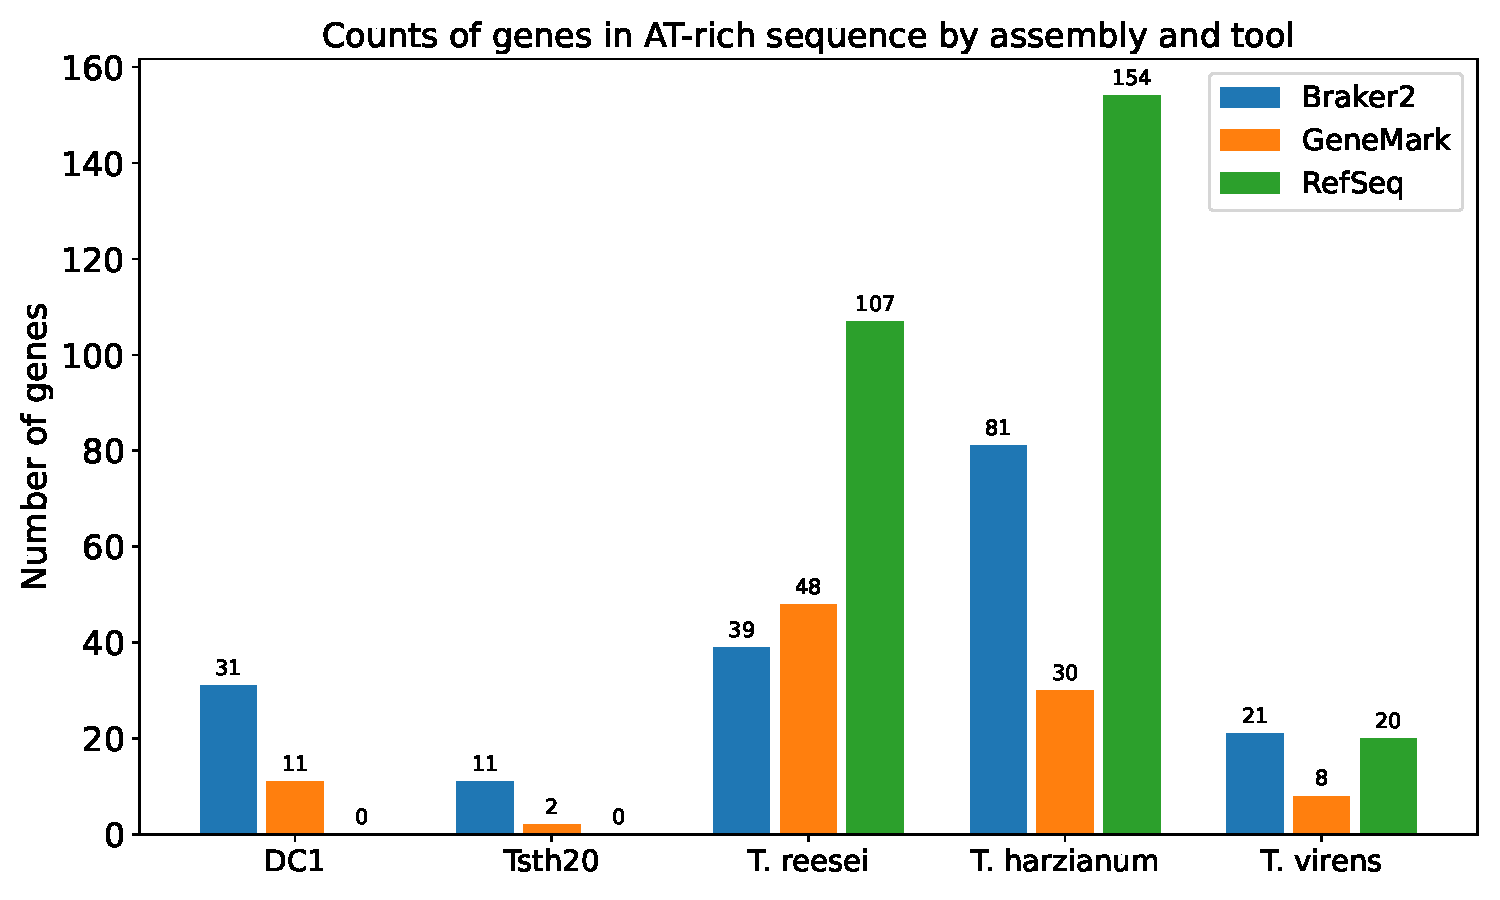
\includegraphics[width=0.90\textwidth]{figures/atrich-genes-barplot.pdf}
  \caption[Gene counts in AT-rich regions]{Number of genes predicted by each gene finder in AT-rich genomic sequence.}
  \label{fig:gc-gene-counts}
\end{figure}

\begin{table}
  \begin{center}
    \begin{tabular}{|c|c|c|c|}
      \hline
      Assembly & Braker2 & GeneMark & RefSeq \\ \hline
      DC1 & 31 & 11 & N/A \\ \hline
      Tsth20 & 11 & 2 & N/A \\ \hline
      \textit{T. reesei} & 39 & 48 & 107 \\ \hline
      \textit{T. harzianum} & 81 & 30 & 154 \\ \hline
      \textit{T.virens} & 21 & 8 & 20 \\ \hline
    \end{tabular}
  \end{center}
  \caption[Number of genes predicted in AT-rich regions]{Number of genes predicted by Braker2, GeneMark and RefSeq
    in AT-rich genomic sequence from each assembly.}
  \label{table:gc-gene-counts}
\end{table}

Finally, to test the probability of any given gene prediction falling
in an AT-rich genomic sequence, a two-sided binomial test was
performed to determine if the number of genes predicted in AT-rich
sequences is proportional to fraction of genomic sequence they
comprise. The null hypothesis in this case is that the number of genes
in AT-rich sequence is proportional to the total AT-rich sequence in
the genome. The results of the test are shown in Table
\ref{table:gc-binomial}. In all cases, it appears that the gene
finding tools selected for this analysis do not predict the same
proportion of genes in AT-rich genomic sequence as in typical genomic
sequence.

\begin{table}
  \begin{center}
    \begin{tabular}{|c|c|c|c|c|c|}
      \hline
      Tool & DC1 & Tsth20 & \textit{T. reesei} & \textit{T. harzianum} & \textit{T. virens} \\ \hline
      Braker2 & $9.56*10^{-181}$ & $1.14*10^{-259}$ & $2.68*10^{-96}$ & $4.05*10^{-140}$ & $1.35*10^{-35}$ \\ \hline
      GeneMark & $5.12*10^{-216}$ & $0.0$ & $5.66*10^{-49}$ & $5.37*10^{-219}$ & $5.31*10^{-35}$ \\ \hline
      RefSeq & N/A & N/A & $1.29*10^{-49}$ & $2.44*10^{-205}$ & $7.40*10^{-33}$ \\ \hline
    \end{tabular}
  \end{center}
  \caption[Binomial test results]{\textit{p}-values produced from a two-sided binomial test
    for each combination of tool and assembly.}
  \label{table:gc-binomial}
\end{table}

In summary, very few regions with gene predictions are present in
AT-rich genomic sequence. Additionally, genes predicted in these
regions tend to be isolated and not supported by other gene finders,
although some agreement is observed. In terms of number of genes
predicted, RefSeq tends to predict the most genes in these AT-rich
regions while GeneMark predicts the fewest. Lastly, the selected gene
finding tools do not predict genes in AT-rich sequences in proportion
to the fraction of genomic sequence they comprise.
